%!TEX program= xelatex
\documentclass[oneside,table]{ntuthesis}
\usepackage{enumerate}
\usepackage{times}
\usepackage{wallpaper}
\usepackage{verbatim}
\usepackage{color}
\usepackage{url}
\usepackage{graphicx,dcolumn,bm}
\usepackage{graphicx}
\usepackage{array}
\usepackage{subfigure}
\usepackage{amsfonts}
\usepackage{amsmath}
\usepackage{amssymb}
\usepackage{array,booktabs,arydshln,xcolor}
\usepackage{indentfirst}
\usepackage{pdfpages}
\usepackage{multirow}
\usepackage{caption}
\usepackage{xcolor}
\usepackage{commath}
\usepackage[sort&compress,numbers]{natbib}
%\usepackage{doi}%<----------
\usepackage{nicefrac}
\usepackage[section]{placeins}
\usepackage{braket}
\usepackage{algorithm}
\usepackage[noend]{algpseudocode}
\usepackage{stackengine}
\usepackage{relsize}

\makeatletter
\def\BState{\State\hskip-\ALG@thistlm}
\makeatother
\newcommand{\rjoin}{\rotatebox[origin=c]{-90}{$\Join$}}
\newcommand\barbelow[1]{\stackunder[1.2pt]{$#1$}{\rule{.8ex}{.075ex}}}
\newcommand\VRule[1][\arrayrulewidth]{\vrule width #1}
\newcommand{\Hamiltonian}{\mathcal{H}}
\newcommand{\rb}{\right}
\newcommand{\lb}{\left}
\newcommand{\nearint}{\sum_{\lb<i,j \rb >}}
\newcolumntype{L}[1]{>{\raggedright\let\newline\\\arraybackslash\hspace{0pt}}m{#1}}
\newcolumntype{C}[1]{>{\centering\let\newline\\\arraybackslash\hspace{0pt}}m{#1}}
\newcolumntype{R}[1]{>{\raggedleft\let\newline\\\arraybackslash\hspace{0pt}}m{#1}}
\definecolor{llblue}{rgb}{0.9000,0.9,1.0}
\DeclareMathOperator{\Tr}{Tr}

% uncomment this if you want to indent the first paragraph
\usepackage{indentfirst}

% uncomment this if you want to make pdf file with hyperlink
\usepackage[colorlinks=false]{hyperref}

\CenterWallPaper{0.174}{watermark.pdf}
\setlength{\wpXoffset}{6.1725cm}
\setlength{\wpYoffset}{10.5225cm}
\setcounter{tocdepth}{4}
\setcounter{secnumdepth}{4}

\makeatletter
\g@addto@macro\normalsize{%
  \setlength\abovedisplayskip{8pt}
  \setlength\belowdisplayskip{8pt}
  \setlength\abovedisplayshortskip{8pt}
  \setlength\belowdisplayshortskip{8pt}
  \setlength{\parskip}{8pt}
}
\makeatother
\hypersetup{
	pdfauthor={Chou, Yun-Hsuan},
	pdftitle={Comparison between Tensor Network Algorithms Appied to Two Dimensional Infinite Quantum Many-Body Systems},
	pdfsubject={Master Thesis}
}


% Using the tex-text mapping for ligatures etc.
\defaultfontfeatures{Mapping=tex-text}

% Set the default fonts
\setmainfont{Times New Roman}
\setCJKmainfont[AutoFakeBold=2,AutoFakeSlant=.4]{DFKai-SB}



% Your information goes here
% author: Tz-Huan Huang [http://www.csie.ntu.edu.tw/~tzhuan]

% ----------------------------------------------------------------------------
% "THE CHOCOLATE-WARE LICENSE":
% Tz-Huan Huang wrote this file. As long as you retain this notice you
% can do whatever you want with this stuff. If we meet some day, and you think
% this stuff is worth it, you can buy me a chocolate in return Tz-Huan Huang
% ----------------------------------------------------------------------------

% Syntax: \var{English}{Chinese}
\university{National Taiwan University}{國立台灣大學}
\collage{College of Science}{理學院}
\institute{Department of Physics}{物理學系}
\title{Comparison between Tensor Network Algorithms for Two Dimensional Infinite Quantum Many-Body Systems}{比較不同張量網路演算法應用在二微多體量子物理系統之優劣}
\author{Yun-Hsuan Chou}{周昀萱}
\studentid{R02222062}
\advisor{Ying-Jer Kao, Ph.D.}{高英哲 博士}
\year{2016}{105}
\month{April}{4}
\day{3}


\begin{document}

\frontmatter

\makecover

%\makecertification
 \newpage
 \thispagestyle{empty}
 \mbox{}
%\includepdf[pages={1}, pagecommand={}]{plots/output.pdf}

\begin{acknowledgementszh}
隨著時光流逝,終於完成了我在物理系的碩班生涯。比起大學在材料系的無聊日子,這三年的經歷讓我感到彌足珍貴。

首先我要感謝高英哲老師的指導與包容。讓比較晚才理解並進入狀況的我也能有機會學習現在十分流行的 Tensor Network 演算法並參與開發 Uni10 的工作,讓我了解在設計CPU與GPU程式時該有的相關資訊與技巧。並在我研究十分掙扎時給予我研究的方向與建議,也讓我有許多機會與其他學者討論以克服問題,對於我的研究有了長足的幫助。

再來是要感謝組上的同學。其中特別感謝謝昀達學長在他繁忙日程裡,仍撥隴指導一個剛開始不怎麼會寫 c/c++ 的菜鳥,並讓我對 Tensor Network 相關的演算法有更進一步的認識。再來我想感謝從未謀面的張學文學長,許許多多研究上的問題,都可以在神秘的玩貝資料夾中得到答案或起發。還要感謝感謝楊淵棨學長、吳柏寬學長、郭子傑學長、李致遠學長、高文瀚、林育平、易德、吳凱析對於我研究與課業上的種種幫助。其中特別感謝吳柏寬學長與林育平,除了對於我在物理理論、學業和娛樂上的幫忙外,也讓本應因研究卡關而在研究室崩潰的夜晚變得十分熱鬧充滿活力,並授與了我二階張亮黑魔導的頭銜。

最後,十分想感謝我的父母。不論我的選擇結果是好與壞、風險高或低,總是不斷地給與我精神上的鼓勵與物質上的支持,感謝你們的包容,才我能讓我毫無顧慮、充實的過完我碩班的時光,體驗著不一樣的人生。
\end{acknowledgementszh}

%\begin{acknowledgementsen}
%I'm glad to thank\ldots 
%\end{acknowledgementsen}

%!TEX root = thesis.tex
\begin{abstractzh}
如何判斷多體量子系統的相變化,在
\end{abstractzh}

\begin{abstracten}
In statistical and condensed matter physics, the phase transition and the critical behavior are very important topics.
\end{abstracten}

\begin{comment}
\category{I2.10}{Computing Methodologies}{Artificial Intelligence --
Vision and Scene Understanding} \category{H5.3}{Information
Systems}{Information Interfaces and Presentation (HCI) -- Web-based
Interaction.}

\terms{Design, Human factors, Performance.}

\keywords{matrix product state(MPS), projected entangled pair state(PEPS), projected entangled simplex state, infinite time-evolveing block-decimation, corner transfer matrix, tensor renormalization group, lBenchmarks, uni10.}
\end{comment}


\tableofcontents
\listoffigures
\listoftables

\mainmatter

% Your thesis goes here
%!TEX root = thesis.tex
\chapter{Introduction}
\label{chapter:Introduction}

\section{Overview}
\label{overview}
	bond dimension is too big to do simulation.



%!TEX root = thesis.tex
\chapter{Tensor Network Theory} 
In this chapter, we will introduce the foundations of tensor network \cite{jordan_studies_2011,Orus2014117,bauer_tensor_2011}, which is a new language for condense matter physics, and explain how to map the quantum many-body systems into the tensor network. 
%This section begins from a fundamental question: How to draw a tensor network diagram? In tensor network theory , we are used to represent tensors as the notations, shown in Fig.~\ref{fig211}, because \textit{tensor diagrams} can fully describe the quantum states of any geometric lattice systems explicitly. Furthermore, base on its clear representation, the implementation of tensor network algorithms become simply. 

\section{Representation of tensors in tensor Networks}
\label{notations}

In mathematical concept, a tensor is considered as a multi-dimensional array of scalars. It could be described by a node and few bonds in the tensor network language. The each bond represent to an \textit{index} of the array, and the number of bonds corresponds to the rank of the tensor. See Fig.~\ref{fig211}(i-iv), the notations without bonds, with a single bond, with two bonds and with $N$ bonds can be considered as scalars, vectors, matrices and rank-$N$ tensors. To explain more clearly, if there is a tensor $T_{\alpha \beta \gamma}$ shown as the Fig.~\ref{fig211}(iv) and the dimensions of the each bond $\alpha, \beta$ and $\gamma$ are $\chi_{\alpha},\chi_{\alpha}$ and $\chi_{\gamma}$, we can say that the tensor $T_{\alpha \beta \gamma}$ contains $\chi_{\alpha}\chi_{\beta}\chi_{\gamma}$ coefficients.

%\begin{align}
%	D_{total} = \begin{cases}
%		1 & \text{, if $N = 0$} \\
%		\chi_{1}\chi_{2}\chi_{3} \dots \chi_{N} & \text{, if $N \neq 0$}
%	\end{cases}
%\end{align}

\begin{figure}[ht]
	\centering
	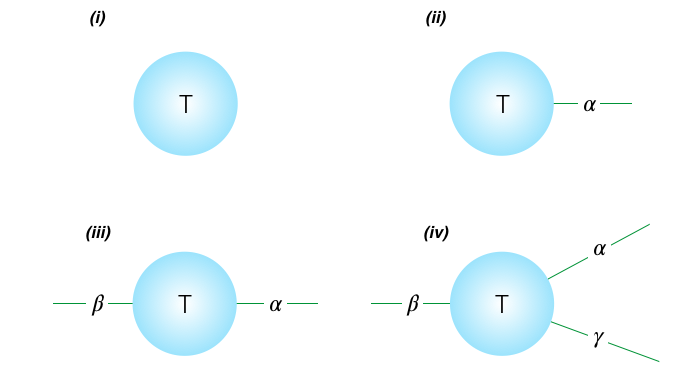
\includegraphics[width=0.75\textwidth]{figures/fig211.png}
	\caption[The reprecentation of commen tensors.]{(i) A tensor without bonds is a scalar $T$, (ii) A tensor with one bond is a vector $T_{\alpha}$, (iii) A tensor with two bonds is a Matrix $T_{\alpha \beta}$, (iv) A tensor with three bonds is a rank-3 tensor $T_{\alpha \beta \gamma}$.}
	\label{fig211}
\end{figure}

\section{Tensor operations and tensor network diagrams} % (fold)
\label{operation}

Since computers can only perform the calculation with matrices, to implement calculations of tensor networks on computers, we need do some operations on tensors, such as permutation and reshape. To explain more explicitly, we define a representation at first,
\begin{enumerate}
	\item $T_{[\alpha \beta], \gamma}$: The bonds $\alpha$ and $\beta$ of a tensor $T$ are grouped. It can be recognized as a matrix, which rows and columns are $\chi_{\alpha}\chi_{\beta}$ and $\chi_{\gamma}$. We will discuss more more details in Sec.~\ref{reshape}
\end{enumerate}

\subsection{Permutation}

The permutation operation is to re-order the arrangement of the coefficients in a tensor according to some specified ordering of the bonds. As shown in Fig.~\ref{fig224}, we permute the tensor $A$ to $\hat{A}$, where the arrangement of the coefficients of the tensor $\hat{A}$ is determined by the assignment $\hat{A}_{\alpha \gamma \beta} = A_{\alpha \beta \gamma}$.

\begin{figure}[H]
	\centering
	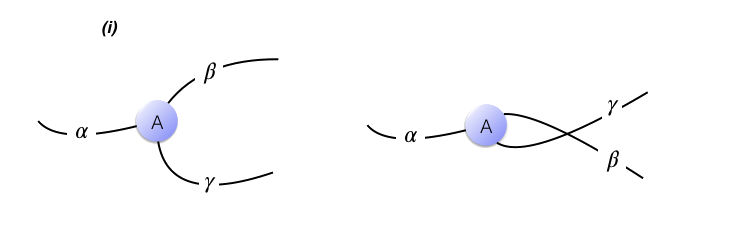
\includegraphics[width=0.75\textwidth]{figures/fig224.png}
	\caption[The permutation of a tensor.]{ Permute tensor $A_{\alpha \beta \gamma}$ to $\hat{A}_{\alpha \gamma \beta}$ }
	\label{fig224}
\end{figure}

\subsection{Reshape}
\label{reshape}
The reshape operation is to combined more than two bonds of a tensor into a single bond. Although the rank of the tensor is reduced, the arrangement of coefficients is unchanged. The dimension of the new bond is equal to the product of the dimensions of the bonds contained in it. As shown in Fig.~\ref{figreshape}, we joint the bonds $\alpha$ and $\beta$ into a new bond $\delta$. Assume that the dimension of the bonds $\alpha$ and $\beta$ are $\chi_{\alpha}$ and $\chi_{\beta}$. The dimension of the bond $\delta$ is equal to $\chi_{\alpha}\chi_{\beta}$.

\begin{figure}[H]
	\centering
	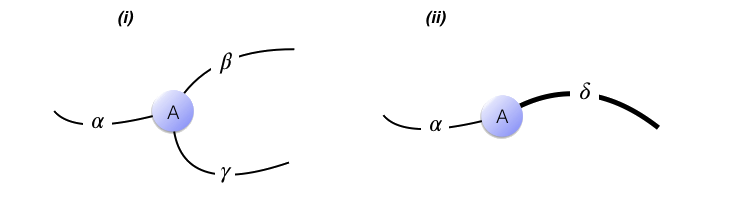
\includegraphics[width=0.75\textwidth]{figures/figreshape.png}
	\caption[The permutation of a tensor.]{ Permute tensor $A_{\alpha \beta \gamma}$ to $\hat{A}_{\alpha \gamma \beta}$ }
	\label{figreshape}
\end{figure}

%\begin{align}
%	A_{\alpha \beta \gamma} \rightarrow \hat{A}_{\alpha \gamma \beta}
%\end{align}

%Nevertheless, the arrangements of tensor $A_{\alpha \beta \gamma}$ is modified to $\hat{A}_{\alpha \gamma \beta}$. The components of them are exact equivalence. 
%
%\begin{figure}[ht]
%	\centering
%	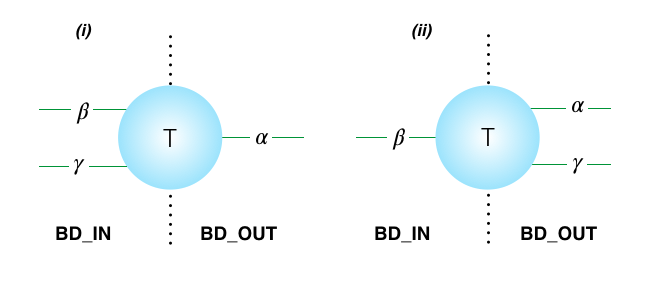
\includegraphics[width=0.80\textwidth]{figures/fig221.png}
%	\caption[Representaion of unfold tensors.]{(i) Unfold a tensor to a matrix $T_{\chi_{\beta}\chi_{\gamma},\chi_{\alpha}}$, (ii) Unfold a tensor to a matrix $T_{\chi_{\beta},\chi_{\alpha}\chi_{\gamma}}$.}
%	\label{fig221}
%\end{figure}

%In order to explain more clearly, we separate the tensor to two part, incoming (BD\_IN) and outgoing (BD\_OUT) which are also designed for distinguishing different types of \textit{uni10::Bond} in \textit{Uni10 Library} \cite{}, to show what the meaning of reshape is in the linear algebra. The total dimensions of the bonds in the part BD\_IN and BD\_OUT corresponds to the number of rows and columns of a matrix. For instance, if the indices of $T_{\alpha \beta \gamma}$ ordered like Fig.~\ref{fig221}(i), $T_{\alpha \beta \gamma}$ is equivalent to a matrix $M_{\chi_{\beta}\chi_{\gamma},\chi_{\alpha}}$, where $\chi_{\alpha}$, $\chi_{\beta}$ and $\chi_{\gamma}$ are the dimensions of the bonds, $\alpha$, $\beta$ and $\gamma$. Similarity, The tensor shown as Fig.~\ref{fig221}(ii) can be recognized as a matrix $M_{\chi_{\beta},\chi_{\alpha}\chi_{\gamma}}$.

\subsection{Tensor contraction}

Tensor contraction is defined as the sum of all products of the shared indices of tensors. For instance, the tensor diagram of contracting two rank-2 tensors $A_{\alpha \beta}$ and $B_{\beta \gamma}$ is shown as Fig.~\ref{fig222}(i) which can be written as
\begin{align}
	C_{\alpha \gamma}=\sum\limits_{\beta = 1}^{\chi_{\beta}}{A_{\alpha \beta}B_{\beta \gamma}},
\end{align}
where $\chi_{\beta}$ is the dimension of the bond $\beta$, and it can be recognized as the inner-product of two matrices $A_{\chi_{\alpha}, \chi_{\beta}}$ and $B_{\chi_{\beta}, \chi_{\gamma}}$. Now that we extend to a more complicated example, see Fig.~\ref{fig222}(ii). The equation of the tensor diagram is described as
\begin{align}
	D_{\alpha \gamma \sigma \epsilon}=\sum_{\beta \rho \delta}{A_{\rho \beta}B_{\beta \sigma \epsilon \delta}C_{\gamma \delta \rho \alpha}}.
\end{align}
In this case, we desired to contract the bonds $\rho,\beta$ and $\delta$ which dimensions are $\chi_{\rho}, \chi_{\beta}$ and $\chi_{\delta}$. Hence, we can complete the contraction processes by following steps,

\begin{figure}[H]
	\centering
	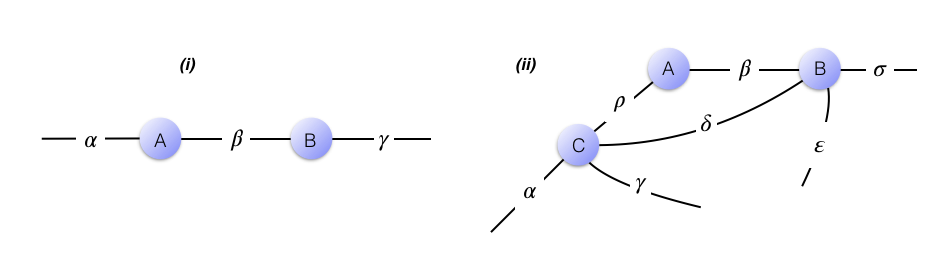
\includegraphics[width=0.75\textwidth]{figures/fig222.png}
	\caption[The examples of tensor diagrams.]{(i) Contract rank-2 tensors $A_{\alpha \beta}$ and $B_{\beta \gamma} $ (ii) Contract a rank-2 tensor $A_{\rho \beta}$, and two rank-4 tensors $B_{\sigma \varepsilon \delta}$ and $C_{\delta \rho \alpha}$}
	\label{fig222}
\end{figure}

\begin{figure}[ht]
	\centering
	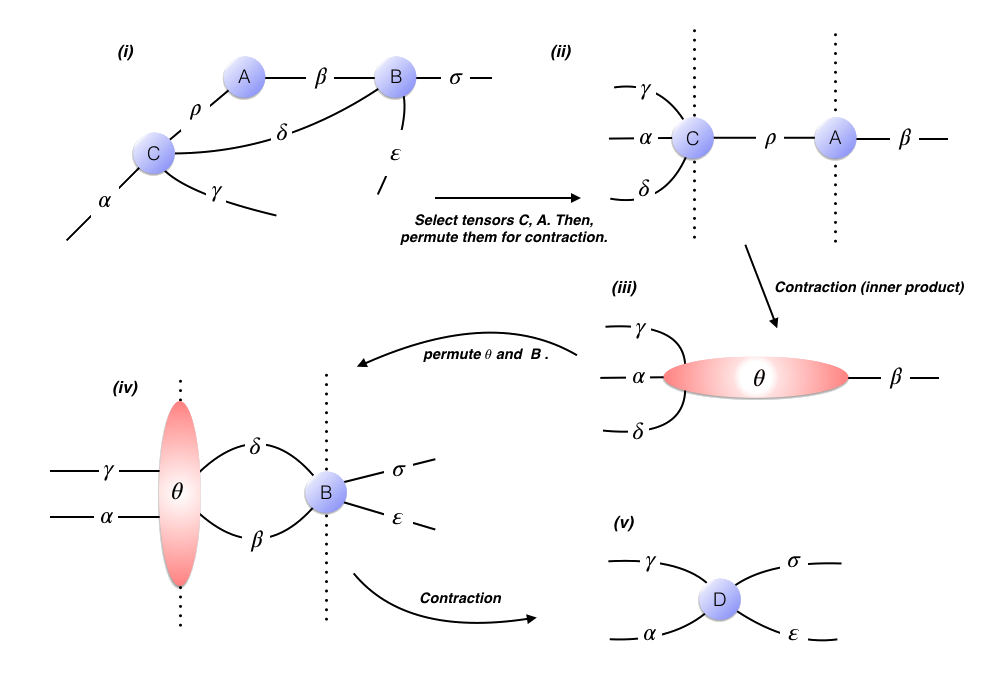
\includegraphics[width=0.75\textwidth]{figures/fig223.png}
	\caption[The contraction procedures of the network shown in Fig\ref{fig222}(ii)]{ The contraction procedures of the network shown in Fig\ref{fig222}}
	\label{fig223}
\end{figure}

\begin{enumerate}

	\item Select a pair of tensors arbitrarily: In the example, we choose the tensor $A_{\rho \beta}$ and $C_{\gamma \alpha \delta \rho}$ at first. 
	\item Permute the tensors to specific shape and operate the inner-product: As shown in Fig.~\ref{fig223}(ii)-(iii) Permute $A_{\rho \beta}$ and $C_{\gamma \alpha \delta \delta}$ to the specified shape $A_{\rho, \beta}$ and $C_{[\gamma \alpha \delta], \rho}$, which can be considered as the inner product of two matrices $A$ and $C$, 
		\begin{align}
			\theta_{\gamma \alpha \delta \beta} = \sum_{\rho = 1}^{\chi_{\rho}}{C_{[\gamma \alpha \delta], \rho} A_{\rho, \beta}}
		\end{align}
	\item Repeat the step (1) and (2) until all tensors are contracted: See Fig.~\ref{fig223}(iii)-(iv), repeat the steps again to contract the remained tensors $\theta_{\gamma \alpha \delta \beta}$ and $B_{\beta \sigma \delta \varepsilon}$
\end{enumerate}
%Actually, the choice in step (1) is restricted in some algorithms, such as corner transfer matrix \cite{PhysRevB.85.205117} and fast full update \cite{PhysRevB.92.035142}, because the order of the contraction network is strongly correlated to the efficiency. For example, if the dimensions of the bonds of the tensors, $A_{\rho \beta}$, $B_{\beta \sigma \epsilon \delta}$ and $C_{\gamma \delta \rho \alpha}$ in Fig.~\ref{fig223}(i), are $D$. The consumption of the contraction of $A_{\rho \beta}$ and $C_{\gamma \delta \rho \alpha}$ is $D^4$. However, if we contract $B_{\beta \sigma \epsilon \delta}$ and $C_{\gamma \delta \rho \alpha}$ at first, it will increase to $D^6$. Therefor, how to determine the cheapest contraction order is a significant issue \cite{PhysRevE.90.033315}.

\section{Describe Quantum states with tensor network} % (fold)
\label{sub:map2quan}

Before drawing a many-body system with tensor-network representation, we should discuss how to describe a spin chain composed by $N$ particles, with each particles having $d$ states. The system can be regard as a congregation of $N$ localized particles and we have recognized that a pure state corresponds to a vector in Hilbert space. Hence, the wave-function of many-body systems can be described by $N$ subspace
\begin{align}
	\Ket{\Psi_{N}} =\sum_{i_1,i_2,\ldots,i_N}{C_{i_1,i_2,i_3,\ldots,i_N}\Ket{i_1}\otimes\Ket{i_2}\otimes \ldots \otimes \Ket{i_N}},
	\label{wavefunc}
\end{align}
where each individual wave function $\Ket{i_1}, \Ket{i_2},\ldots, \Ket{i_N}$ has the degree of freedom $d$. After writing down the formulation of the wave-function, Eq.~\ref{wavefunc}, we are able to build a tensor-network representation for quantum states. The wave-function $\Ket{\Psi_N}$ is shown as Fig.~\ref{fig225}(a), each bond of the tensor corresponds to the local Hilbert space $\Ket{i_n}$ and the dimension of it is equivalent to the probable states of the particles on the $n$-th site and the coefficients of the rank-$N$ tensor corresponds to $C_{i_1,i_2,i_3,\ldots,i_N}$.

No matter from Eq.~\ref{wavefunc} or Fig.~\ref{fig225}(i), we can notice that the number of coefficients in $C_{i_1,i_2,i_3,\ldots,\i_N}$ is proportional to $d^N$, directly. Therefor, it is impossible to fully describe a many-body system by a classical machine if the system size larger than fifty. Fortunately, according to the theory of MPS \cite{PhysRevB.73.094423} \cite{PhysRevLett.75.3537}, the wave-function can be decomposed to two subsystem by the Schmidt decomposition.
\begin{figure}[ht]
	\centering
	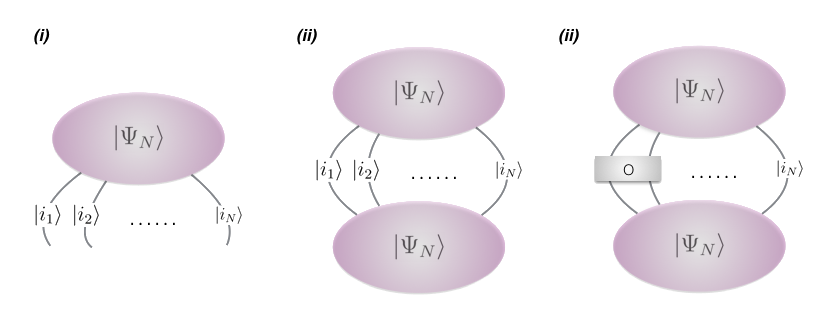
\includegraphics[width=0.75\textwidth]{figures/fig225.png}
	\caption[Represent wave-function of quntum states of TN]{(i) The wave-function, $\Ket{\Psi_N}$ (ii) The norm of $\Ket{\Psi_N}$, $\Braket{\Psi_N|\Psi_N}$ (iii) Expectation value of observable $O$, $\Bra{\Psi_N}O\Ket{\Psi_N}$}
	\label{fig225}
\end{figure}

\section{Matrix product state}
\label{MPS}

Base on the theory of MPS, the wave-function composed by pure states can be decompose to many unit cells by \textit{sigular value decomopostion} and \textit{Schmidt decomposition}. To explain the MPS structure more explicitly, we begin from splitting the wave-function $\Ket{\Psi_N}$ [Fig.~\ref{fig225}(a)] between $n$ and $n+1$ sites with Schmidt decomposition, 
\begin{align}
	\label{schmitwave}
	\Ket{\Psi_{N}} = \sum_{\alpha_n} \lambda_{\alpha_n} \Ket{\psi_{\alpha_n}^{[1\dots n]}} \Ket{\psi_{\alpha_n}^{[n+1\dots N]}}
\end{align}
where $\lambda_{\alpha_n} > 0$ and $\sum\limits_{\alpha_n}{\lambda_{\alpha_n}^2 = 1}$. To obtain the one site wave function $\Ket{\psi_{\alpha_n}^{[n+1]}}$, we perform Schmidt decomposition on $\Ket{\psi_{\alpha_n}^{[n+1\dots N]}}$ between the $n+1$ and $n+2$ sites,
\begin{align}
	\Ket{\psi_{\alpha_n}^{[n+1\dots N]}} = \sum_{\alpha_{n+1}} \lambda_{\alpha_{n+1}} \Ket{\psi_{\alpha_{n+1}}^{[n+1]}} \Ket{\psi_{\alpha_{n+2}}^{[n+2\dots N]}}
\end{align}
then span $\Ket{\psi_{\alpha_{n+1}}^{[n+1]}}$ by the spin basis $i_{n+1}$,
\begin{align}
	\Ket{\psi_{\alpha_{n+1}}^{[n+1]}} = \sum_{i_{n+1}}{\Gamma^{[n+1] i_{n+1}}_{\alpha_n \alpha_{n+1}} \Ket{i_{n+1}}}
\end{align}
and the Eq. \ref{schmitwave} can be re-written as, 
\begin{align}
	\Ket{\Psi_{N}} = \sum_{\alpha_n,\alpha_{n+1}}\sum_{i_{n+1}}{\lambda_{\alpha_n} \Gamma^{[n+1] i_{n+1}}_{\alpha_n \alpha_{n+1}} \lambda_{\alpha_{n+1}l} \Ket{\psi_{\alpha_n}^{[1\dots n]}} \Ket{i_{n+1}} \Ket{\psi_{\alpha_{n+2}}^{[n+2\dots N]}} }
\end{align}
In the end, we can repeat the same process site-by-site in the entire system and obtain the MPS structure,
\begin{align}
	\Ket{\Psi_N} = \sum_{\alpha_1,\dots ,\alpha_N}\sum_{i_1,\dots ,i_N}{ \Gamma^{[1] i_{1}}_{\alpha_1} \lambda_{\alpha_1} \Gamma^{[2] i_{2}}_{\alpha_1 \alpha_{2}} \lambda_{\alpha_2} \dots  \lambda_{\alpha_{N-2}} \Gamma^{[N-1] i_{N-1}}_{\alpha_{N-2} \alpha_{N-1}} \lambda_{\alpha_{N-1}} \Gamma^{[N] i_{N}}_{\alpha_{N}} \Ket{i_1 i_2 \dots i_N}}
\end{align}
and the tensor network representation is shown as Fig.~\ref{fig311}, 
\begin{figure}[ht]
	\centering
	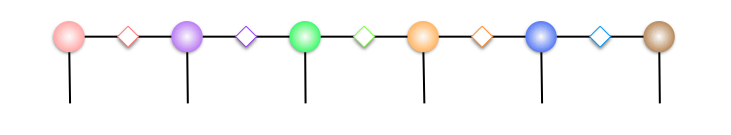
\includegraphics[width=0.90\textwidth]{figures/fig3111.png}
	\caption[The tensor network representation of matrix product states]{The tensor network representation of matrix product states.}
	\label{fig311}
\end{figure}

Now that we try to expand it to a infinite chain \cite{PhysRevLett.98.070201}. Since the translation invariance, the wave function $\Ket{\Psi_{N=\infty}}$ can be represent as $n$-site translational symmetric states, which means that $\Gamma^{[i]}$ and $\lambda^{[i_{i}]}$ are independent of $\Gamma^{[i+n]}$ and $\lambda^{[i+n]}$. For instance, when $n=2$, the wave-function of a infinite chain can be recognized as a composite of two different matrix product states $\lambda^{[A]}\Gamma^{[A]}$ (red nodes) and $\lambda^{[B]}\Gamma^{[B]}$ (purple nodes), as shown in Fig.\ref{fig312}, 

\begin{figure}[ht]
	\centering
	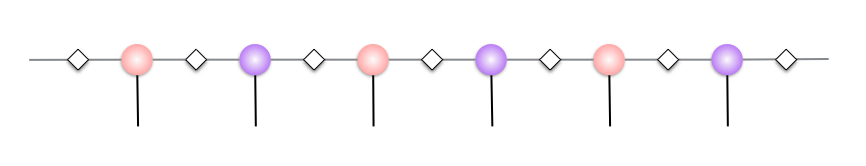
\includegraphics[width=0.90\textwidth]{figures/fig311.png}
	\caption[The tensor network representation of infinite matrix product states]{The tensor network representation of infinite matrix product states.}
	\label{fig312}
\end{figure}

Next, in order to update the two states in the unit cell, we utilize the \textit{Suzuki Trotter decomposition} to approximate the entire evolution operator with $2$-sites operators, \textit{The first-order Suzuk-Trotter decompostio} of operator $e^{\delta (A+B)}$ is,
\begin{align}
	\label{STd}
	e^{\delta A + B} = e^{\delta A}e^{\delta B} + O(\delta^2)
\end{align}
where $A$ and $B$ are two non-commutative operators.Therefore, the entire evolution operator can be approximated by grouping the two site operator $H_{AB}$ and $H_{BA}$,
\begin{align}
	\label{evoopt}
	e^{-\tau H} = \left(e^{-\delta H}\right)^{\frac{\tau}{\delta}} \approx \left(\prod e^{\delta H_{AB}} \right)\left( \prod e^{\delta H_{BA}}\right)
\end{align}
and we can obtain the evolution operator $e^{H_{AB}}$ and $e^{H_{BA}}$ straightly after solving two-site hamiltonians, $H_{AB}$ and $H_{BA}$.
So far, we have constructed the infinite MPS and the 2-site evolution operators $e^{-\tau H_{AB}}$ and $e^{-\tau H_{BA}}$. Hence, the tensor network representation of Eq.~\ref{mapgroud} can be drawn as Fig.~\ref{fig313}, which means that the ground state $\Ket{\psi_0}$ can be regard as contracting all the tensors in the diagram. So the next problem: How can we contract them and preserve the structure like Fig{\ref{fig311}}?

\begin{figure}[ht]
	\centering
	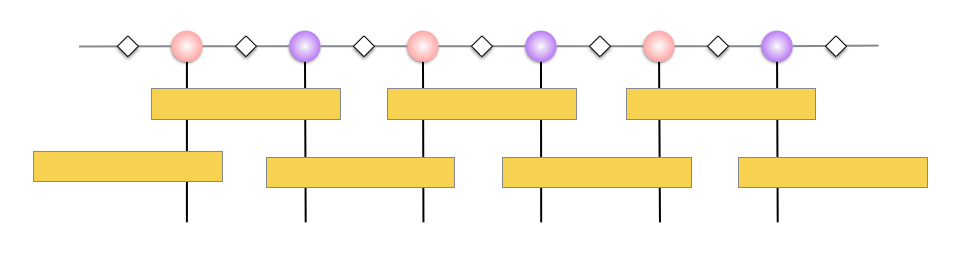
\includegraphics[width=0.90\textwidth]{figures/fig312.png}
	\caption[The tensor diagram of imaginary time evolving block decimation.]{The red and blue tensor denote on \textit{odd} and \textit{even} sites and the yellow tensors are time evolution operators $e^{-\tau H_{AB}}$ and $e^{-\tau H_{BA}}$}
	\label{fig313}
\end{figure}


%!TEX root = thesis.tex
\chapter{2-D Imaginary Time Evolving Block Decimation}
\label{chapter:2ditebd}

In this chapter we introduce some different ways to implement two-dimensional imaginary time-evolving block decimation and apply them in calculation of ground state of Heisenberg and transverse Ising model on two-dimensional square lattice. In section \ref{ite} and \ref{itebd}, we briefly review the idea of imaginary time evolution (iTEBD),[\ref{vidal}] and explain how to extend it to two-dimensional [\ref{X,zhon}]. Second, we briefly review another method to make 2D-iTEBD more stable[\ref{1.1}]. In the last section \ref{2dopt}, we record various particulars which are helpful optimizing algorithms.

\section{Imaginary Time Evolution}
\label{ite}
Theoretically, if having the imaginary time evolution operator $e^{-\tau H}$, we could project any random states to the ground state, as long as the wave-function can be written as,
\begin{align}
	\label{mapgroud}
	\Ket{\psi_0} = \frac{e^{\tau H} \Ket{\Psi}}{\parallel e^{\tau H} \Ket{\Psi}\parallel}
\end{align}
but according to the eq.\ref{mapgroud}, we may found that the number of coefficients in an origin evolution operator $e^{-\tau H}$ is proportional to $2^N \times 2^N$. On the other words, it is impossible to update entire system directly. In order to restricting the rapid dimensional growth, we apply \textit{Suzuki Trotter decomposition}[\ref{1.1}][\ref{1.1}] to approximate. The main idea of \textit{Suzuki Trotter} is decomposing the whole system to lots of units cell and using some smaller operations to update the wave-function.
\begin{align}
	\label{STd}
	e^{\delta A + B} = e^{\delta A}e^{\delta B} + O(\delta^2)
\end{align}
eq.\ref{STd} means the first-order Suzuki Trotter  decomposition, and A and B are non-commutative with each other.

Now that the dimension of the evolution operator is reduced to a n-site operator and in chapter \ref{chapter:properties}, we have shown that a many-body system can map to a MPS or PEPS structure, so we can draw the process of updating a ground state like Fig.\ref{fig312},

\begin{figure}[ht]
	\centering
	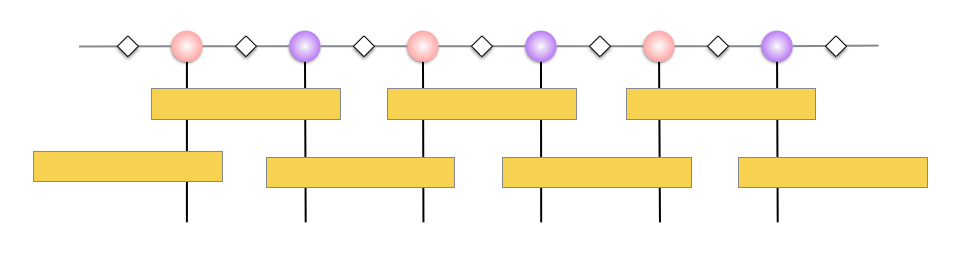
\includegraphics[width=0.75\textwidth]{figures/fig312.png}
	\caption[The picture of the main idea of itebd.]{The red and blue tensor denotes on \textit{odd} and \textit{even} sites. The yellow one are time evolution operators $e^{-\tau H_{k,k+1}}$, $e^{-\tau H_{k+1,k}}$}
	\label{fig312}
\end{figure}

On the other work, contract the tensors in Fig.\ref{fig312} repeatedly until the ground state energy to the minimum. The remained tensor is considered as the ground state of the system. So the next question: How can we contract them and preserve the structure like Fig{\ref{fig311}}? This answer is iTEBD.

\begin{figure}[ht]
	\centering
	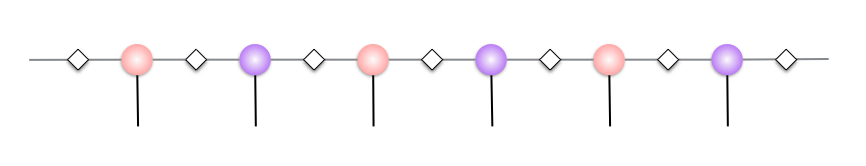
\includegraphics[width=0.75\textwidth]{figures/fig311.png}
	\caption[The picture of matrix product states]{The simple form of a matrix product state.}
	\label{fig311}
\end{figure}

\section{Simple Infinite Imaginary-Time Evolving Block Decimation for 2-D system}
In this section, we apply the TN diagrams to introduce the methods of implementation of algorithm. If you are interested in the mathematical formula of them, please read the references \citep{vidal_efficient_2004} [\ref{dd}][\ref{eaef}], witch include more details of theoretical discussion.

\label{itebd}
\subsection{Simple Description of iTEBD for 1-D system}

The algorithm start from 2 random states and 2 random diagonal matrices which are considered as entanglement between particles. In the TN diagrams, Fig.\ref{fig313}, the states and entanglement between neighbor sites are represented by the nodes and bonds with different colors.

\label{1ditebd}
\begin{figure}[ht]
	\centering
	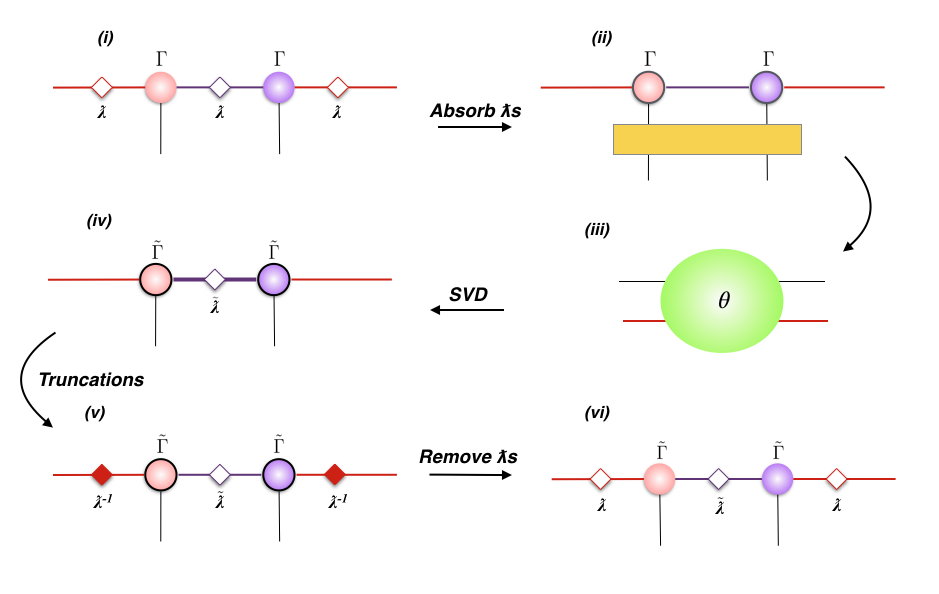
\includegraphics[width=0.90\textwidth]{figures/fig313.png}
	\caption[The tensor network diagrams for the 1-D iTEBD]{ (i)Absorb all $\lambda$ to $\Gamma$. (ii) Contract an evolution operator $e^{-\delta H}$ for evolving the system. (iii) Decompose the tensor $\theta$ by SVD. (iv) Truncate and Update the states and $\lambda$ on the green bond.(v) Remove $
		\lambda$ for obtaining the states. (iv) After updating the states and $\lambda$ on the purple bond, apply the way to update the red bond and repeat all the steps until the ground state convergence.}
	\label{fig313}
\end{figure}

The processes shown in Fig.\ref{fig313} is a standard strategy for implementation of iTEBD and also called \textit{Simple Update}. 

In one dimensional system, the performance of Simple Update is pretty well, because 1-D systems obey the canonical form and have less influences of environment. However, in 2-D systems, due to the area law, we need consider the environment more restrictively when measuring the local observable. Moreover, the computational consumption is another serious problem, owing to the growth of a state's dimension which is proportional to $dD^4$.

In order to solving that obstacles, optimizations of 2-D algorithms  became an important part in condense matter physics. This chapter we focus on obtaining good enough projected entangled pair states from 2-D iTEBD and the strategies of improving measurement would be shown in following chapters.

\subsection{Description and Pseudocode of iTEBD for 2-D system}
\label{2ditebd}

Now that we stated to extend it to a two dimensional system. In chapter.\ref{chapter:properties}, we have known that a two dimensional many-body system is able to be represented by PEPS. Due to impossibly drawing an network of infinite sites, the structure of infinite PEPS (iPEPS) is decided by the geometry of the lattice and the unit cell we chosen. In usual, the size of unit cell depend on the n-site evolution operator. For instance, if the target is updating iPEPS of a square lattice with 2-site operator, the tensor diagram would be drawn as Fig.\ref{fig314}.

\begin{figure}[ht]
	\centering
	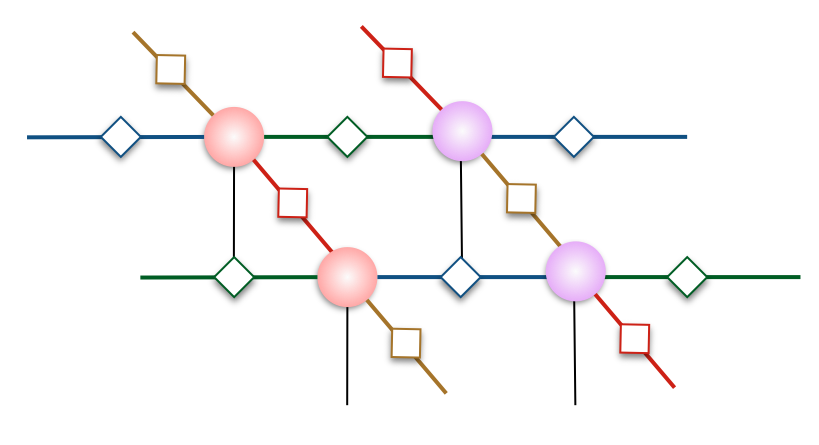
\includegraphics[width=0.6\textwidth]{figures/fig314.png}
	\caption[The tensor diagrams of 2-D lattice]{Four sites unit cell in iPEPS.}
	\label{fig314}
\end{figure}

After setting the form of iPEPS, we start to deal the question of updating states. The most intuitive scheme is to apply the scheme of \textit{Simple Update} which is shown in Fig.\ref{fig315}. The steps are similar to the iTEBD on 1-D systems. However, there are some differences. Firstly, the projected entangled pair states is a rank-5 tensor. Secondly, there are more entangled should be considered, due to increased neighbor sites.

More theoretical descriptions are written in [\ref{}][\ref{}]. Here, we explain the methods with TNs and some simple pseudocodes. The basic idea of \textit{2-D iTEBD} is to update the states from four directions by \textit{Simple Update}. The example starting from updating the green bond is shown in Fig.\ref{fig315} and Fig.\ref{fig316},

\begin{figure}[ht]
	\centering
	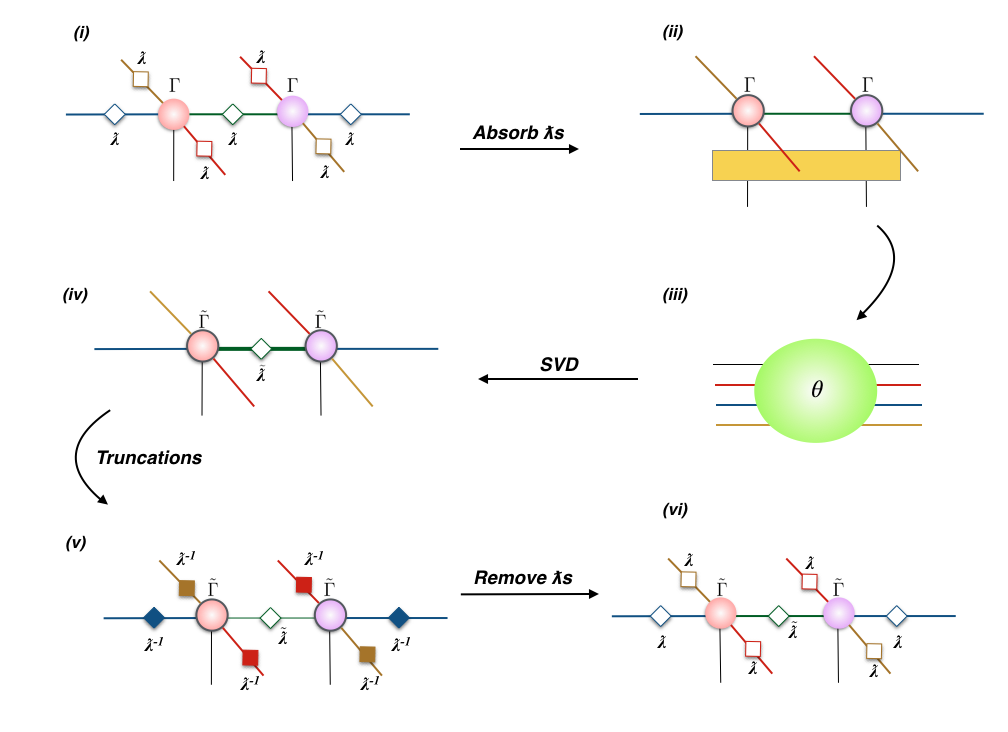
\includegraphics[width=1.00\textwidth]{figures/fig315.png}
	\caption[The tensor network diagrams of updating the green bond in iPEPS with 2D-iTEBD]{Absorb all $\lambda$ to $\Gamma$. (ii) Contract an evolution operator $e^{-\delta H}$ for evolving the system. (iii) Decompose the tensor $\theta$ by SVD. (iv) Truncate and Update the states and $\lambda$ on the green bond.(v) Remove $\lambda$ for obtaining the states. (iv) Obtain a original form of iPEPS. Repeat all the step to update the other bonds until the ground state energy convergence}
	\label{fig315}
\end{figure}

It's the same as one dimensional case, The first step is to absorb all $\lambda$ around the sites. The tensor with gray bold means the state have absorbed all entanglements. Secondly, contract the gate, $e^{-\delta H}$, for getting the tensor $\theta$. Thirdly, apply singular value decomposition to update states and the entanglement on the green bond. After decomposing $\theta$, we found that the dimension of the green bond increase to $dD^4$. Therefor, truncation plays a significant roles for keeping the dimension in the algorithm. In the end of the updating processes, multiply pseudo inverse of all $\lambda$ to the tensors for reducing to original form. 

	\begin{figure}[ht]
	\centering
	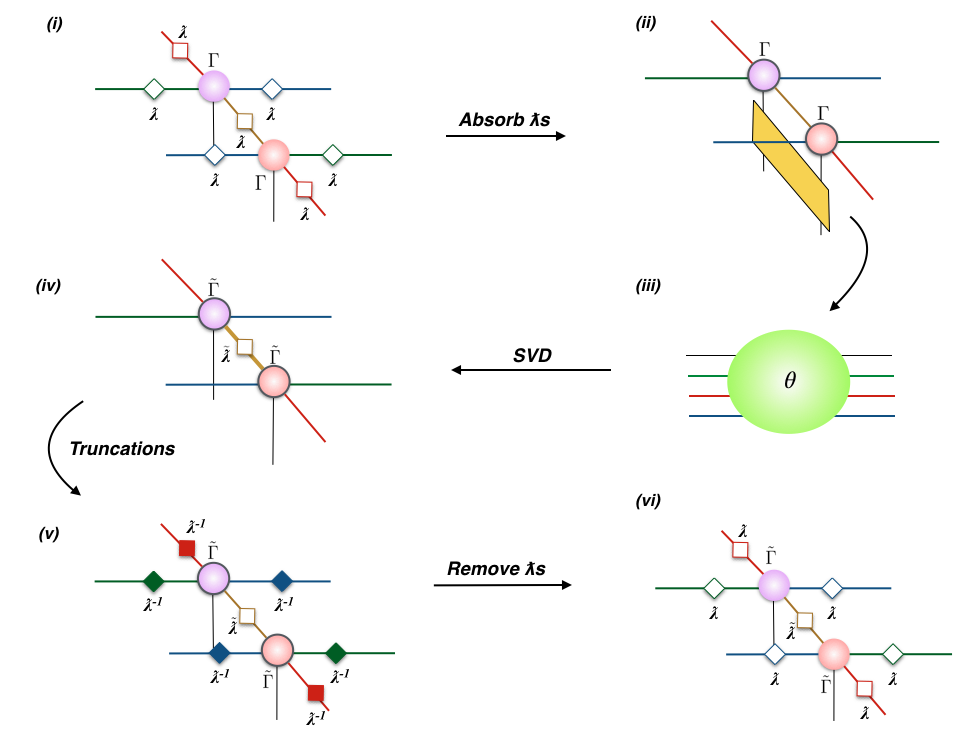
\includegraphics[width=1.00\textwidth]{figures/fig316.png}
	\caption[The tensor network diagrams of updating the yellow bond in iPEPS with 2D-iTEBD]{Update the yellow bond and the steps are similar to Fig.\ref{fig315}}
	\label{fig316}
	\end{figure}

	For easily to imagine how to updating the others directions. The updating steps of yellow bond are shown In Fig.\ref{fig316}.

%\begin{algorithm}
%	\caption{My algorithm}\label{euclid}
%	\begin{algorithmic}[1]
%		\Procedure{MyProcedure}{}
%		\State $\textit{stringlen} \gets \text{length of }\textit{string}$
%		\State $i \gets \textit{patlen}$
%		\BState \emph{top}:
%		\If {$i > \textit{stringlen}$} \Return false
%		\EndIf
%		\State $j \gets \textit{patlen}$
%		\BState \emph{loop}:
%		\If {$\textit{string}(i) = \textit{path}(j)$}
%		\State $j \gets j-1$.
%		\State $i \gets i-1$.
%		\State \textbf{goto} \emph{loop}.
%		\State \textbf{close};
%		\EndIf
%		\State $i \gets i+\max(\textit{delta}_1(\textit{string}(i)),\textit{delta}_2(j))$.
%		\State \textbf{goto} \emph{top}.
%		\EndProcedure
%	\end{algorithmic}
%\end{algorithm}


\section{Ameliorate two-dimensional iTEBD}
\label{2dhastin}

This method which make the algorithm more stable was published by \textit{M. B. Hastings}. Although \textit{Simple Update} shown in section.\ref{2ditebd} can obtain pretty good states, it's not stable and efficient enough. The reason is that too many multiplications of pseudo inverse $\lambda$ at the step Fig.\ref{fig315}(v). In numerical methods, it's hard to deal the problem of dividing the value which is equal or approach to zero. On the other words, the more inverse operations, the more the probability of bring about divergence or destroying algorithms.

For reducing the risk of breaking algorithms. Firstly, declare the states $\Gamma$ which include two entanglements among them. For instance, In Fig.\ref{fig317}(i), the red tensor is considered as multiplication of $A$ and the $\lambda$ on the yellow. The purple one is multiplication of $B$ and remained $\lambda$. Secondly, in Fig.\ref{fig317}(ii), because the entanglements on red and blue bonds are included in tensor $B$, we just need absorb the yellow one and contract the evolution operation for obtaining tensor $C$. Thirdly, we contract the red and blue $\lambda$ to the red and blue bonds which belong to the original tensor $A$ in tensor $C$ for getting $\theta$. Fourthly, getting the $\tilde{B}$ from decomposing and truncating $\theta$. Owing to avoid multiplying inverse matrices, we get $\tilde{A}$ by contracting tensor $C$ and $\tilde{B}$ and multiply an inverse $\lambda$ of yellow bond for removing the entanglement and reducing to original form.

	\begin{figure}[ht]
	\centering
	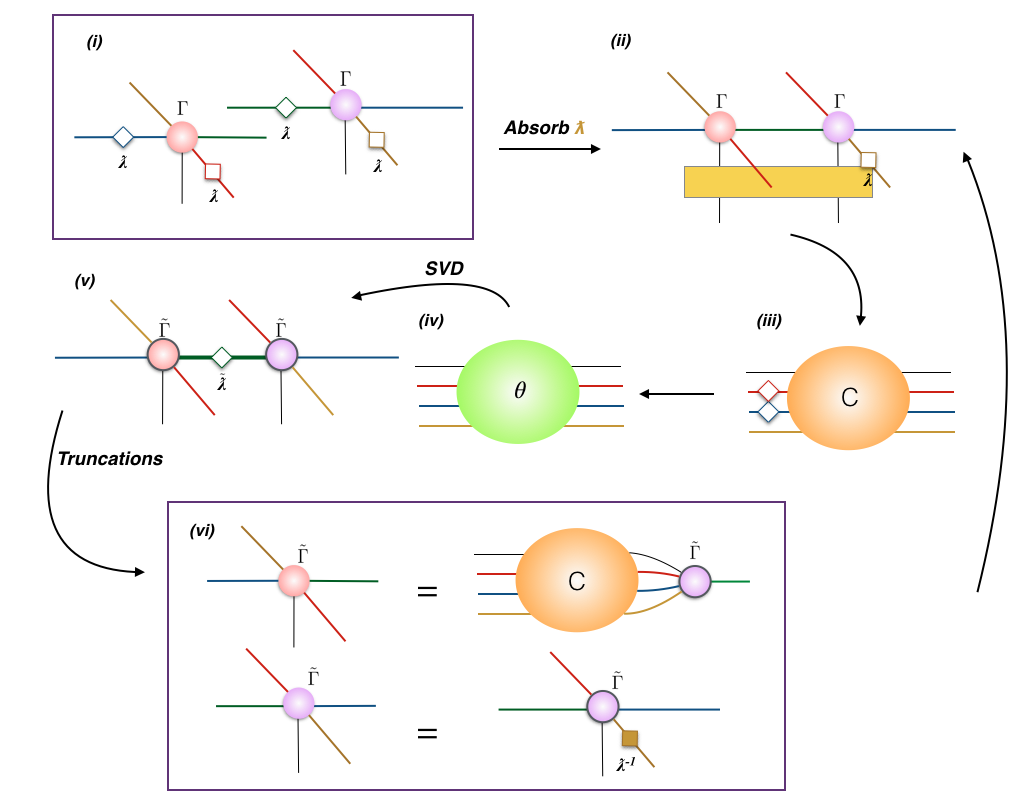
\includegraphics[width=1.00\textwidth]{figures/fig317.png}
	\caption[The tensor network diagrams for the 2-D iTEBD with QR decomposition]{The tensor network diagrams for the ameliorated 2-D iTEBD.}
	\label{fig317}
	\end{figure}

	Finally, repeat all the processes shown in Fig.\ref{fig317} to update different bonds until the convergence of the ground state energy.

\section{Optimizations}
\label{2dopt}

\subsection{Initialization}
\label{2doptInit}
Intuitively, the initialization of states should not affect the result. However, it's a serious misunderstanding. Actually, stating from a awful initial sates may break the algorithms or hardly converge.

From the viewpoint of physics, translational invariance is one of essential properties in many-body system, So we can assume that the group state on two sites should be similar. For instance, if the TN diagram of the states is shown as Fig \ref{fig321}(i), Fig \ref{fig321}(ii) might be the better way to initialize the states.

\begin{figure}[ht]
	\centering
	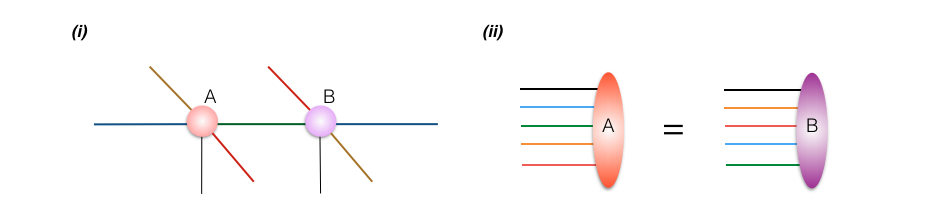
\includegraphics[width=1.00\textwidth]{figures/fig321.png}
	\caption[The diagrams of initializing projected entangled pair states]{(i) The structure of PEPS, (ii) The initialization of states}
	\label{fig321}
\end{figure}

\subsection{Truncattion Error}

\subsection{QR decomposition}

Though the strategy described in previous sections improve the stability, it's not efficient enough. The reason why is that the dimension of tensor $\theta$, in Fig.\ref{fig315}(iii) and Fig.\ref{fig317}(iii), is proportional to $d^2D^6$. In addition to that, the time complexity of singular value decomposition is proportional to $O(NM^2)$. In conclusion, the steps, in Fig.\ref{fig315}(iii) and Fig.\ref{fig317}(iii), are expensive, it is necessary to reduce the dimension of tensor $\theta$. 
\label{2doptQR} \begin{figure}[H] \centering 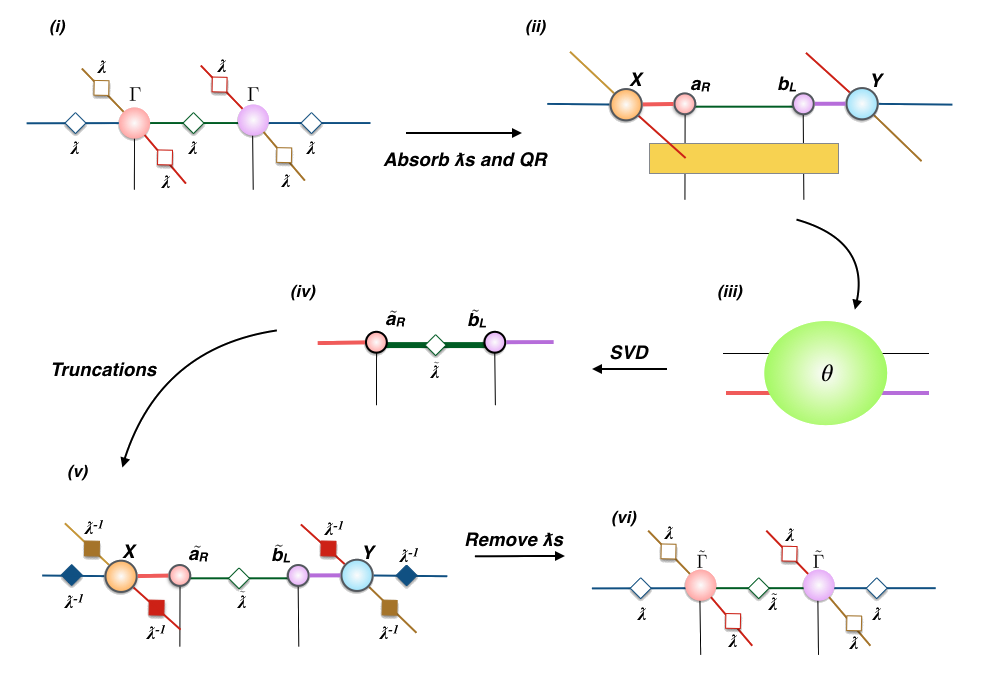
\includegraphics[width=0.80\textwidth]{figures/fig318.png} \caption[The tensor network diagrams for the ameliorated 2-D iTEBD with QR decompositiont]{The tensor network diagrams for the ameliorated 2-D iTEBD.} \label{fig318} \end{figure} To achieve the goal, the projected pair state must be decomposed by QR decomposition. The processes making \textit{Simple Update} more efficient is illustrated in Fig \ref{fig318}.  Most of the steps shown in Fig \ref{fig318} are like in Fig \ref{fig315}. The only difference is that after absorbing all the $\lambda$, we decompose the state to an orthogonal matrix and an upper triangular matrix by QR. For instance, in Fig \ref{fig318} (ii), the state $A$ is decomposed to an orthogonal matrix X and upper triangular matrix $a_R$. Due to the columns of $X$ are orthonormal, $XX^{\dagger}$ is equal to $I$. In the other word, the tensor $X$ can be ignored and we just need consider the tensor $a_R$ by QR. Similarity, the state $B$ can be decomposed to a lower triangular $b_L$ and an orthogonal matrix $Y$ by LQ which is equivalence to operate QR decomposition after transpose the matrix. Next, (iii) we can obtain the tensor $\theta$ whose dimension is $d^2D$ from $a_R$, $b_L$ and an evolution operator.

\begin{figure}[ht]
	\centering
	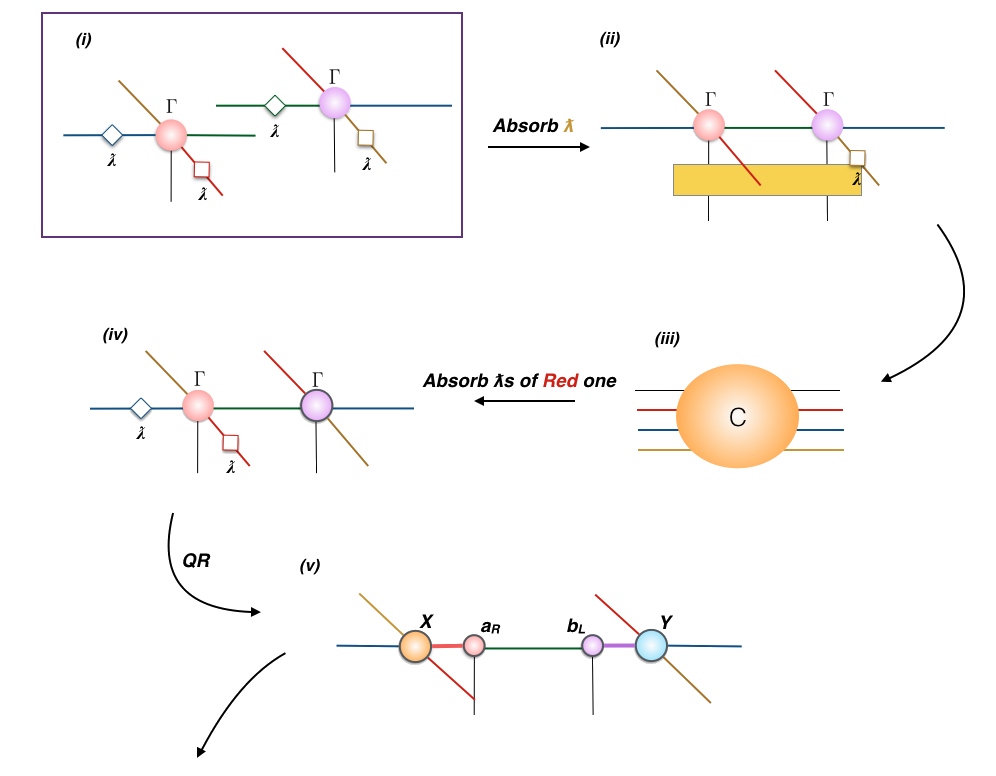
\includegraphics[width=0.90\textwidth]{figures/fig319.png}
	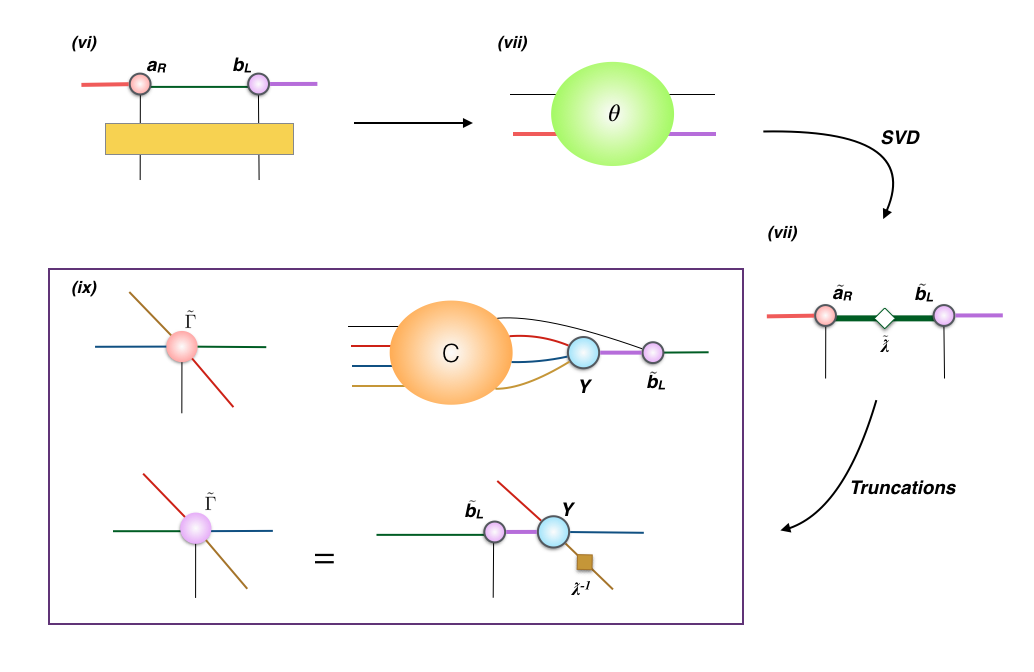
\includegraphics[width=0.90\textwidth]{figures/fig320.png}
	\caption[The tensor network diagrams for the ameliorated 2-D iTEBD with QR decompositiont]{The tensor network diagrams for the ameliorated 2-D iTEBD.}
	\label{fig319}
\end{figure}

The strategy to accelerate \textit{Ameliorate Simple Update} is shown in the Fig \ref{fig319} and its main idea is also to reduce the dimension of $\theta$.

\section{Comparison}

So far, we have benchmarked the improved iTEBD. 

\label{Comparison}
\subsection{Different Initializations}

\begin{figure}[ht]
	\centering
	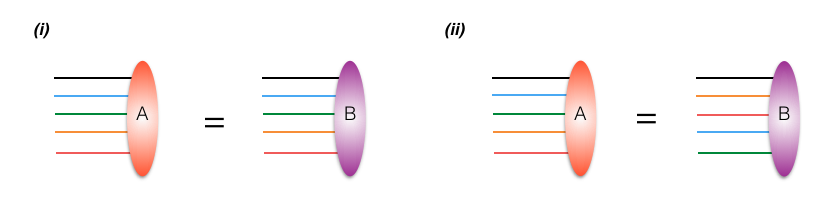
\includegraphics[width=1.00\textwidth]{figures/fig322.png}
	\caption[Different methods to initialize the states]{(i) Type 1, (ii) Type 2}
	\label{fig322}
\end{figure}

See Fig \ref{fig323}, the both cases are 

\begin{figure}[ht]
	\centering
	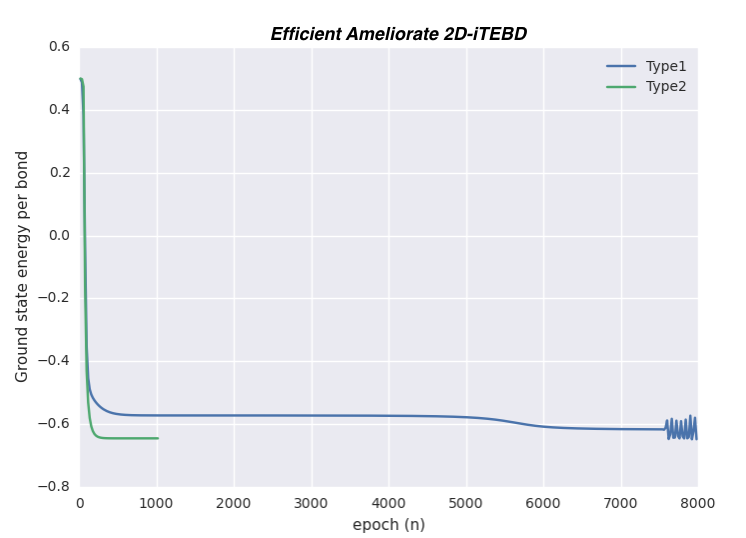
\includegraphics[width=0.75\textwidth]{figures/fig323.png}
	\caption[Comparison the results of Heisenberg model on square lattice which are obtaining from different initial states.]{The Blue line represents updating tensors from the initial state shown in Fig \ref{fig322} (i) and the green one represents updating from Fig \ref{fig322} (ii)}
	\label{fig323}
\end{figure}

\begin{figure}[ht]
	\centering
	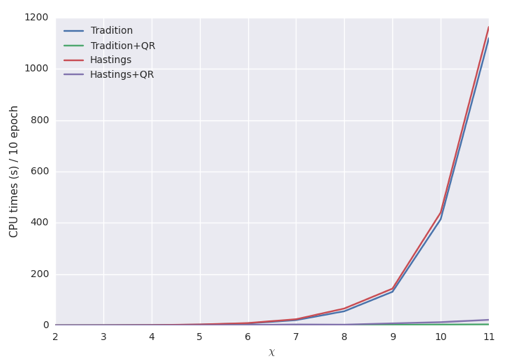
\includegraphics[width=0.75\textwidth]{figures/fig324.png}
	\caption[tmp]{}
	\label{fig324}
\end{figure}

\begin{figure}[ht]
	\centering
	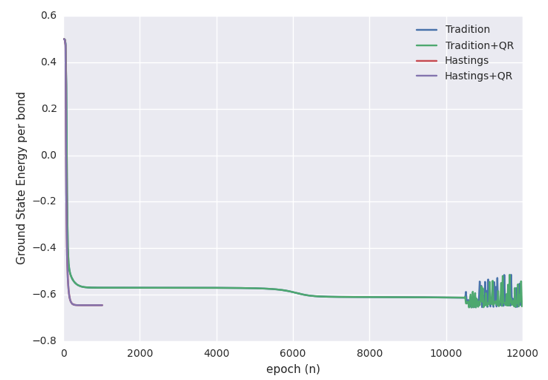
\includegraphics[width=0.75\textwidth]{figures/fig325.png}
	\caption[tmp]{}
	\label{fig325}
\end{figure}

\begin{figure}[ht]
	\centering
	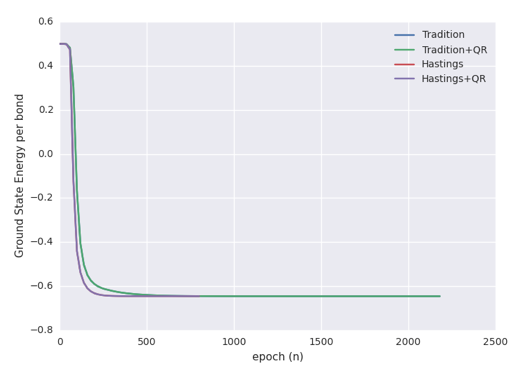
\includegraphics[width=0.75\textwidth]{figures/fig326.png}
	\caption[tmp]{}
	\label{fig326}
\end{figure}

\begin{figure}[ht]
	\centering
	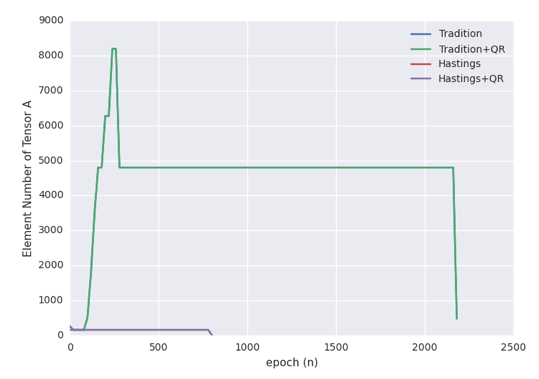
\includegraphics[width=0.75\textwidth]{figures/fig327.png}
	\caption[tmp]{}
	\label{fig327}
\end{figure}

%!TEX root = thesis.tex
\chapter{Infinite Projected Entangled Simplex State}
\label{chapter:ipess}

\section{Infinite Kagome Lattice}
\subsection{3-PESS}
\label{3pess}

\subsection{5-PESS}
\label{5pess}

\section{Infinite Square Lattice}
\subsection{4-PESS (local tensors are rank-2)}
\label{4pess2b}
\subsection{4-PESS (local tensors are rank-4)}
\label{4pess4b}


%!TEX root = thesis.tex
\chapter{Corner Transfer Matrix}
\label{chapter:ctm}
The \textit{cerner transfer matrix renormalization group} (CTMRG) \cite{doi:10.1143/JPSJ.65.891} \cite{PhysRevB.80.094403} \cite{PhysRevB.84.041108} is an algorithm to numerically compute the \textit{effective environments} which is an approximation of the environment of systems. For example, if the infinite PEPS is composed by a single tensor $A^{h}_{uldr}$ repeatedly, where $h$ express a physical basis of  $\mathbb{V}$ with dimension $d$, and $u,l,d,r$ are virtual bonds with dimension $D$, see Fig.~\ref{fig501}(a). Then we can represent the scale norm $\Braket{\psi|\psi}$ by a simple two dimensional tensor network $\varepsilon$ which is characterized by reduced tensors $a$, shown in Fig.~\ref{fig501}(b). The reduced tensor $a$ is defined as eq.\ref{reduce_a}, 
\begin{align}
	\label{reduce_a}
	a \equiv \sum_{h=1}^{d} A_{h} \otimes A^{*}_{h}
\end{align}
The environment $\varepsilon^{[\vec{r}]}$ of the site $\vec{r}$ could be described by the reduced tensors in the gray rectangles in Fig.\ref{fig501}(c) and the \textit{effective environments} $G^{[\vec{r}]}$ shown in Fig.~\ref{fig501}(d) is target of the CTMRG. 

In the following subsections, we will show more details of implementation of CTM and compare some features between obtaining the states from iPEPE and PESS.

\begin{figure}[ht]
	\centering
	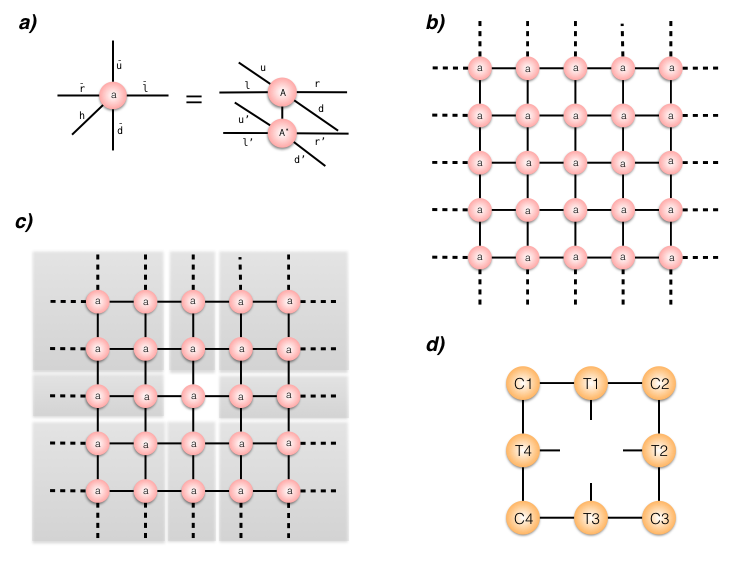
\includegraphics[width=0.75\textwidth]{figures/fig501.png}
	\caption[The tensor diagrams of the corner transfer matrix with the one-site unit cell.]{The tensor diagrams of corner transfer matrix. (a) The reduced tensor $a$ is obtained from the iPEPS state $A$, where $a \equiv \sum_{h=1}^{d} A_{h} \otimes A^{*}_{h}$. (b) An infinite two-dimensional tensor network $\varepsilon$ . (c) The environment $\varepsilon^{[\vec{r}]}$of the site $\vec{r}$. (d) The effective environment $G^{[\vec{r}]}$.}
	\label{fig501}
\end{figure}

\section{Obtain States from PEPS}
\label{2ditebdctm}
In chapter.\ref{chapter:2ditebd}, we have discussed about obtaining the infinite PEPS state $\Ket{\psi}$ of an infinite 2D square lattice by imaginary time evolution and known that the infinite PEPS could be characterized by two tensors $A^h_{uldr}$ and $B^h_{drul}$ repeatedly (Fig.~\ref{fig511}(a)). The scalar norm of the iPEPS $\Braket{\psi|\psi}$ is composed by reduced tensors $a_{\bar{u}\bar{l}\bar{d}\bar{r}}$ and $b_{\bar{d}\bar{r}\bar{u}\bar{l}}$(Fig.~\ref{fig511}(b)), where
\begin{align}
	\label{reduce_a}
	\bar{a} \equiv \sum_{h=1}^{d} A_{h} \otimes A^{*}_{h} \\
	\label{reduce_b}
	\bar{b} \equiv \sum_{h=1}^{d} B_{h} \otimes B^{*}_{h}
\end{align}

Then, we can consider the environment $\varepsilon^{\left[\vec{r_1},\vec{r_2},\vec{r_3},\vec{r_4}\right]}$ of a four-site structure (Fig.~\ref{fig511}(c)), and try to approximate it with effective environment $G^{\left[\vec{r_1},\vec{r_2},\vec{r_3},\vec{r_4}\right]}$ (Fig.~\ref{fig511}(d)), which consists of $C_1, T_{a1}, T_{b1},C_2, T_{a2}, T_{b2},C_3, T_{a3}, T_{b3},C_4, T_{a4}, T_{b4},$

\begin{figure}[ht]
	\centering
	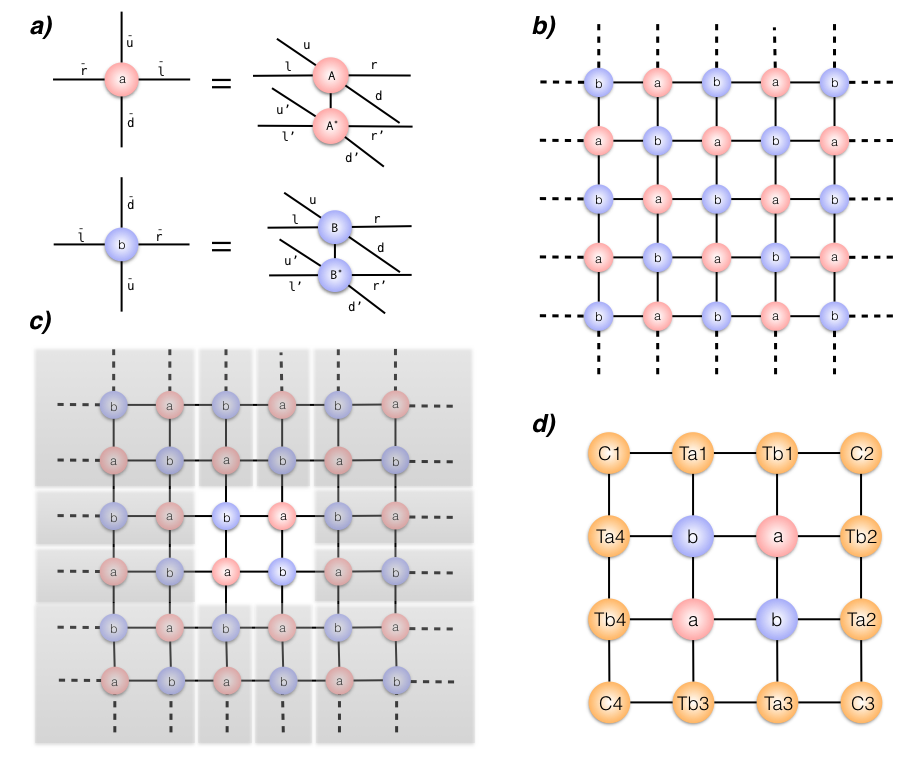
\includegraphics[width=0.75\textwidth]{figures/fig511.png}
	\caption[The tensor diagrams of the corner transfer matrix with the four-site unit cell.]{The tensor diagrams of the corner transfer matrix with the four-site unit cell.(a) The reduced tensor $a$ and $b$ are obtained from the iPEPS state $A$ and $B$, where $a \equiv \sum_{h=1}^{d} A_{h} \otimes A^{*}_{h}$ and $b \equiv \sum_{h=1}^{d} B_{h} \otimes B^{*}_{h}$. (b) An infinite two-dimensional tensor network $\varepsilon$. (c) The environment of the four-site unit cell. (d) The effective environment $G^{\left[\vec{r_1},\vec{r_2},\vec{r_3},\vec{r_4}\right]} = \{ C_1, T_{a1}, T_{b1},C_2, T_{a2}, T_{b2},C_3, T_{a3}, T_{b3},C_4, T_{a4}, T_{b4}\}$.}
	\label{fig511}
\end{figure}

For the approximation of environment, the directional variant of the CTMRG was developed. According to \textit{directional coarse-graining moves}, the effective environment could be updated from four different moves , left, right, up and down and iterated until the environments converges. 

For instance, the procedures to the left move, shown in the Fig.~\ref{fig512} which is derived by Roman and Vidal, is made up of four major steps,
\begin{enumerate}
	\item Insertion: Insert two new columns which consist of \{ $T_{a1},b,a,T_{b3}$ \} and \{ $T_{b1},a,b,T_{a3}$ \} as in Fig.~\ref{fig512}(b).
	\item Absorption: In order to obtaining two new corner matrices $\tilde{C_1}$ and $\tilde{C_4}$, and two new transfer matrices $\tilde{T_{b4}}$ and $\tilde{T_{a4}}$, we contract tensors $C_1$ and $T_{b1}$, tensors $C_3$ and $T_{a3}$, tensors $T_{a4}$ and $b$, and tensors $T_{b4}$ and $a$. Then, contract tensors $\tilde{C_1}$ and $\tilde{T_{b4}}$, and tensors $\tilde{C_4}$ and $\tilde{T_{a4}}$, obtaining $\tilde{Q_1}$ and $\tilde{Q_4}$ which play significant rules for calculating isometries between $\tilde{T_{b4}}$ and $\tilde{T_{a4}}$ as in Fig.~\ref{fig512}(c).
	\item Renormalization: Truncate the vertical virtual bonds of $\widetilde{C_1}$, $\widetilde{T_{b4}}$, $\widetilde{T_{a4}}$, and $\widetilde{C_4}$ by contracting the isometries $Z$ and $W$, where
\begin{align}
	\label{isometry}
	&Z^{\dagger}Z = I \\
	&W^{\dagger}W = I
\end{align}
and the renormalization of the left CTM, yield as
\begin{align}
	\label{renormalize}
	&C^{\prime}_1 = Z^{\dagger} \tilde{C_1} \\
	&T_{b4}^{\prime} = Z\tilde{T_{b4}}W^{\dagger} \\
	&T_{a4}^{\prime} = W\tilde{T_{b4}}Z^{\dagger} \\
	&C^{\prime}_4 = Z\widetilde{C_4}
\end{align}
See the Fig.~\ref{fig512}(d) and \ref{fig512}(f).
	\item Truncation: To determinate the isometries Z and W in the \textit{renormalization} steps is the most significant part. In this case, we use the eigenvalue decomposition of 
		\begin{align}
			\label{eigh_ctm}
			&\tilde{C_1}\tilde{C^{\dagger}_1}+\tilde{C_4}\tilde{C^{\dagger}_4}= \tilde{Z} D_z \tilde{Z^{\dagger}}\\
			&\tilde{Q_1}\tilde{Q^{\dagger}_1}+\tilde{Q_4}\tilde{Q^{\dagger}_4}= \tilde{W} D_w \tilde{W^{\dagger}}
		\end{align}
		shown in Fig.~\ref{fig512}(e). It's not hard to find that the 
		the dimension of bonds of $D_z$ and $D_w$ increase to $\chi^2$. For that reason, we have to truncate $\tilde{Z}$ and $\tilde{W}$ to isometries $Z$ and $W$ which are equivalent to keeping the columns of $\tilde{Z}$ and $\tilde{W}$ corresponding to $\chi$ largest eigenvalues of $D_z$ and $D_w$.
\end{enumerate}

Now, we need repeat the procedures in Fig.~\ref{fig512}(b)-(d) again for absorbing the other inserted column in Fig.~\ref{fig512}(d) and obtain a new effective environment $G^{\prime \left[\vec{r_1},\vec{r_2},\vec{r_3},\vec{r_4}\right]}$ for the four-site unit cell. By composing four variant moves of the CTM we build an epoch of CTMRG. 

\begin{figure}[ht]
	\centering
	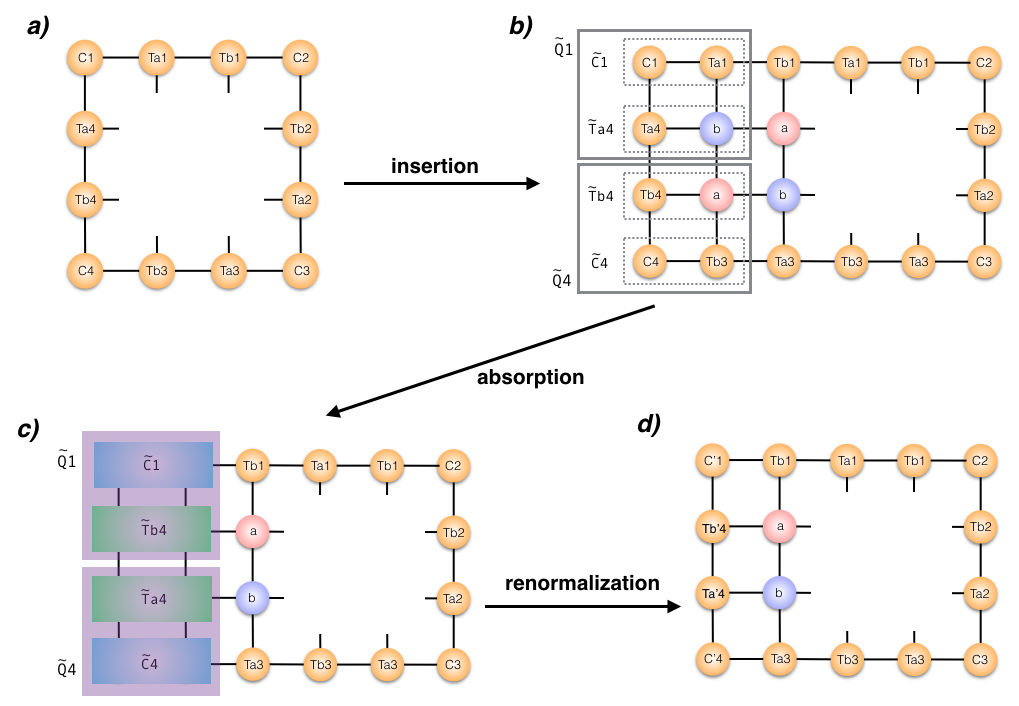
\includegraphics[width=0.80\textwidth]{figures/fig512.png}
	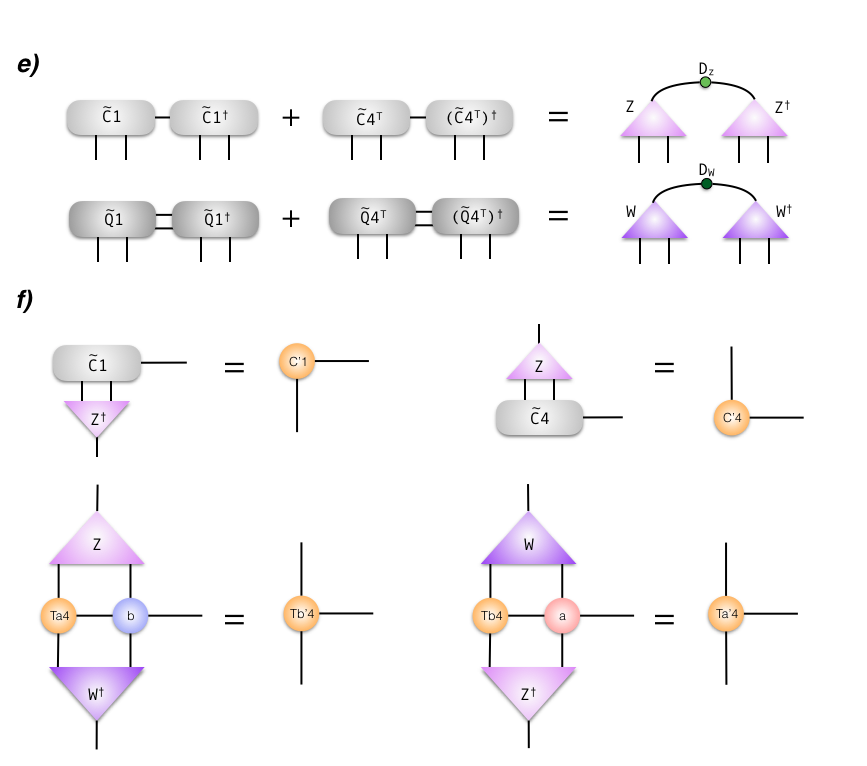
\includegraphics[width=0.80\textwidth]{figures/fig513.png}
	\caption[The procedures of the corner transfer matrix.]{The procedures of the corner transfer matrix. The more discussions are derived in the paragraph}
	\label{fig512}
\end{figure}

\section{Obtain States from PESS}
\label{pessctm}
In this section, we apply the CTM to approximate the effective environment of 4-PESS structure. Firstly, we must transform it to iPEPS structure which is suit for the form of CTM. As shown in Fig.~\ref{fig521}, the projection tensors, $U^{[0]}$, $U^{[1]}$, $U^{[2]}$ and $U^{[3]}$, and the entangled simplex tensors, $S^{[\alpha]}$ and $S^{[\beta]}$ are obtained from 4-PESS ansatz. To map these states to PEPS-like structure, we group the tensors, $S^{[\alpha]}$, $U^{[0]}$ and $U^{[1]}$, in red rectangles into the tensor $A$, 
\begin{align}
	A^{\sigma_i \sigma_j}_{i^{\prime}j^{\prime}kl} = \sum_{ij}{U^{[0]}_{ ii^{\prime},\sigma_i} S^{[\alpha]}_{ijkl} U^{[1]}_{ jj^{\prime},\sigma_j}}
\end{align}
and group, $S^{[\beta]}$, $U^{[2]}$ and $U^{[3]}$, in blue rectangles into the tensor $B$
\begin{align}
	B^{\sigma_k \sigma_l}_{i^{\prime}j^{\prime}kl} = \sum_{k^{\prime}l^{\prime}}{U^{[2]}_{ kk^{\prime},\sigma_i} S^{[\beta]}_{i^{\prime}j^{\prime}k^{\prime}l^{\prime}} U^{[3]}_{ ll^{\prime},\sigma_j}}
\end{align}
, whee the ranks of tensor $A$ and $B$ are six and there are two physical bonds contained in each of them. Hence, after combined the physical bonds in tensors $A$ and $B$, the iPEPS structure will be obtained,
\begin{align}
	A^{\sigma_i \sigma_j}_{i^{\prime}j^{\prime}kl} \rightarrow  A^{\sigma_A}_{i^{\prime}j^{\prime}kl} \\
	B^{\sigma_k \sigma_l}_{i^{\prime}j^{\prime}kl} \rightarrow  B^{\sigma_B}_{i^{\prime}j^{\prime}kl}
\end{align}
Next, in order to make the structure more balance, the entanglement should be well-distributed between each sites, 
\begin{align}
	\widetilde{A} = \sum_{i^{\prime}j^{\prime}kl}{\lambda^{[\beta]^{\frac{1}{2}}}_{i^{\prime}} \lambda^{[\beta]^{\frac{1}{2}}}_{j^{\prime}} A^{\sigma_A}_{i^{\prime}j^{\prime}kl}\lambda^{[\alpha]-\frac{1}{2}}_{l} \lambda^{[\alpha]^{-\frac{1}{2}}}_{k}}\\
	\widetilde{B} = \sum_{i^{\prime}j^{\prime}kl}{\lambda^{[\alpha]^{\frac{1}{2}}}_{k} \lambda^{[\alpha]^{\frac{1}{2}}}_{l} B^{\sigma_B}_{i^{\prime}j^{\prime}kl} \lambda^{[\beta]^{-\frac{1}{2}}}_{i} \lambda^{[\beta]^{-\frac{1}{2}}}_{j^{\prime}}}
\end{align}
and substitute $\widetilde{A}$ and $\widetilde{B}$ into Eq. \ref{reduce_a} and Eq. \ref{reduce_b} to obtain reduced tensors $a$ and $b$. In the end, we apply these two reduced tensor to build the form of CTM and follow the procedures shown in Fig.~\ref{fig512} to simulate the effective environment tensors.

\begin{figure}[ht]
	\centering
	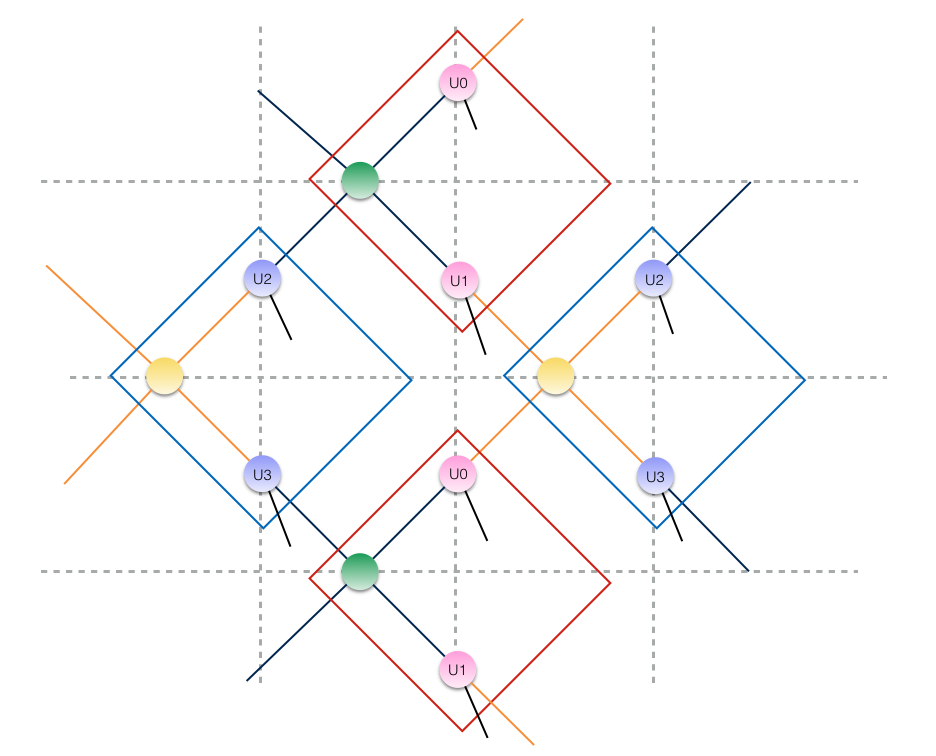
\includegraphics[width=0.70\textwidth]{figures/fig521.png}
	\caption[The tensor diagram of obtaining the reduce tensors from 4-PESS structure.]{The tensor diagram of obtaining the reduce tensors from 4-PESS structure. The reduce tensor $a$ and $b$ are composed by the tensors in the red and blue rectangles}
	\label{fig521}
\end{figure}

\section{Comparison}

To compare the performance of the approximations, we have applied 2D-iTEBD and PESS to approach the ground state of the spin-1/2 quantum transverse Ising model, 
\begin{align}
	H = -\sum_{<\vec{r},\vec{r}^{\prime}>}{\sigma_z^{[ \vec{r}^{} ]} \sigma_z^{[ \vec{r}^{\prime} ]}} - \lambda \sum_{\vec{r}}{\sigma_x^{[ \vec{r} ]}}
\end{align}
, and use directional CTM to obtain the effective environment at each sides. See Fig.~\ref{fig522}, the order-parameter $m_z \equiv  \Bra{\Psi} \sigma_z \Ket{\Psi}$ as a function of the external magnetic field $\lambda$. We find that when measuring the local observable with directional CTM, the better ground states are obtained. However, it have no improvement when approaching to near-critical point. The possible reason is that 
the original states computed by iPEPS approximation is not accuracy sufficiently. Next, turn to the cases which states are obtained from 4-PESS algorithm.When $D=2$ and $\chi = 20$, we find that it is hard to converge near the critical point because the virtual bonds dimension too small to describe the systems. After increasing the virtual dimension, we notice that it converge to $\lambda_c \approx 3.220$. In Sec.~\ref{chapter:ipess}, we have shown that the ground states obtained by 4-PESS has more accuracy. Hence, it is not astonish that the result compute with 4-PESS+CTM is better than 2D-iTEBD+CTM. However, it still can not compare with  the quantum Monte Carlo estimation which is $\lambda^{MC}_c \approx 3.044$ \cite{PhysRevE.66.066110}.

\begin{figure}[H]
	\centering
	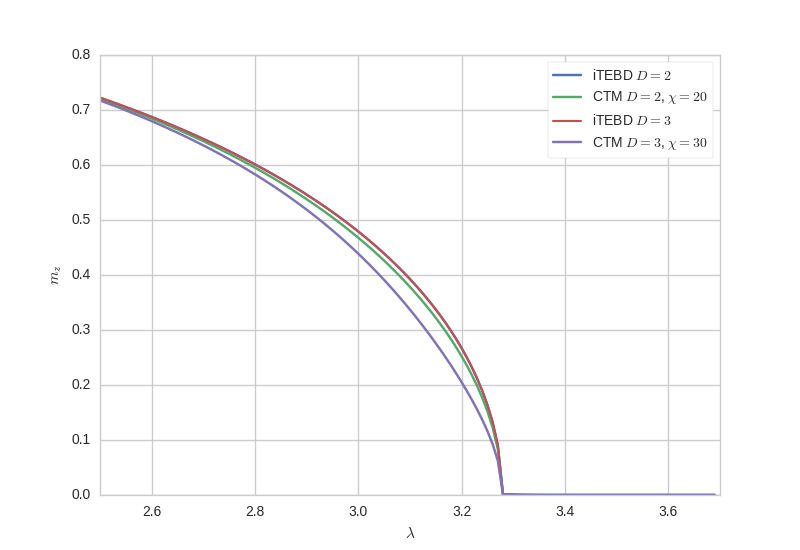
\includegraphics[width=0.75\textwidth]{figures/ctm_itebd.png}
	\caption[Compare the order-parameter $m_z$ of the transfer Ising model on square lattice between 2D-iTEBD and 2D-iTEBD+CTM.]{Compare the order-parameter $m_z$ of the transfer Ising model on square lattice between 2D-iTEBD and 2D-iTEBD+CTM, where the order-parameter $m_z$ as a function of the external field $\lambda$}
	\label{fig522}
\end{figure}

\begin{figure}[H]
	\centering
	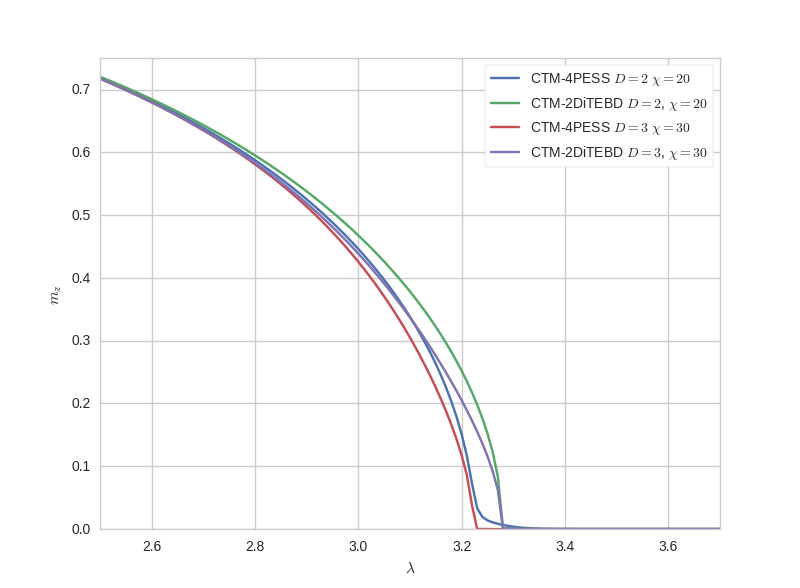
\includegraphics[width=0.75\textwidth]{figures/ctm_pess.png}
	\caption[Compare the order-parameter $m_z$ of the transfer Ising model on square lattice between 2D-iTEBD+CTM and 4-PESS+CTM.]{Compare the order-parameter $m_z$ of the transfer Ising model on square lattice between 2D-iTEBD+CTM and 4-PESS+CTM, where the order-parameter $m_z$ as a function of the external field $\lambda$}
	\label{fig523}
\end{figure}



%!TEX root = thesis.tex
\chapter{Summary}
\label{chapter:summary}

In this thesis, we reviewed the concept of matrix product states (MPS) and drew the structure with tensor diagrams, where the virtual bond dimension $\chi$ between each sites represent that how many the basis and the entanglement information are kept. Next, we introduced the imaginary time-evolving block decimation algorithm (iTEBD), which is the most simple tool to obtain the ground states of the MPS structure. In one dimensional system, the performance of iTEBD have been proved stable and efficient, because it obeys the canonical form and have less influences by environment. 

Owing to the success of 1D-iTEBD, we tried to utilize it to simulate the two dimensional systems. However, we encountered some problems. Firstly, due to the area law, we need consider the environment more restrictively when measuring the local observables. Secondly, the growth of computational consumption to describe project entangled pair states (PEPS) is too high because the dimension of each states is proportional to $dD^4$, where $D$ is the dimension of virtual bonds in PEPS.

Therefore, optimizing two-dimensional algorithms becomes important. In Sec.~\ref{chapter:2ditebd}, we started from basic simple update which is unstable due to multiplying to many pseudo-inverse entangled matrices. Next, to improve the stability of 2D-iTEBD, the new simulation schemes was developed by Hastings. However, these two methods are not applicable to study two-dimensional systems with large bond dimensions because the dimension of the projected tensor $\Theta$ is $d^2D^6$ and the cost CPU time will grow exponentially. Hence, we had better applied the decomposition tools, LQ and RQ, to reduce the dimension of the tensor $\Theta$ from $d^2D^6$ to $d^4D^2$ and it will improve the efficiency effectively. Finally, we have noticed that the ways to initialize the states and setting a suitable cutoff $\varepsilon$ to determine how many basis should be truncated have a certain impact on the accuracy and stability of the algorithms. 

Then, in Sec.~\ref{chapter:ipess}, we have introduced another method, project entangled simplex state (PESS) ansatz, to obtain the ground states in two-dimensional systems. Instead of containing the entangled information between each sites, we applied $n$-rank tensors to describe the entanglement in simplices. In conclusion, the computational consumption is less than PEPS ansatz because the dimension of the states on each sites is reduced to $dD^2$ and can obtain the ground states more accurately in strongly correlated and frustrated systems, such as kagome and Husimi lattices. However, in square lattice systems, the PESS ansatz is not only hard to converge but also unstable and even break down in the end.

Finally, we reviewed the corner transfer matrix (CTM) to consider the influences of the environment. In conclusion, the accuracy will be improved when we measure the local observable with effective environment. However, so far we still can not simulate the environment with large virtual bond dimension $D$ simply because the dimension of the reduce tensors is proportional to $D^8$, which means that the consumption and the required simulation time would increase exponentially. To deal with this problem, we have developed the open source library, Uni10, which not only make the implementation of tensor network algorithms more convenient but also can be easily accelerated with GPU.



\appendix

\addcontentsline{toc}{chapter}{\bibname}
%\bibliographystyle{unsrtnat}
\bibliographystyle{apsrev4-1}
%\bibliographystyle{plainnat}
%\bibliographystyle{apalike}

% Your bibliography goes here

\bibliography{thesis}

%\makespine
\end{document}
